\chapter{A19 管理者只追求可衡量的东西} % Introduction chapter suppressed from the table of contents



\hypertarget{ux4e0dux77e5ux9053ux5e94ux8861ux91cfux4ec0ux4e48ux7684ux7ba1ux7406ux8005ux53eaux80fdux8ffdux6c42ux53efux8861ux91cfux7684ux4e1cux897f}{%
\section{不知道应衡量什么的管理者只能追求可衡量的东西}\label{ux4e0dux77e5ux9053ux5e94ux8861ux91cfux4ec0ux4e48ux7684ux7ba1ux7406ux8005ux53eaux80fdux8ffdux6c42ux53efux8861ux91cfux7684ux4e1cux897f}}

(51 Managers who don't know how to measure what they want settle for
wanting what they can measure.)

\framebox{%
\begin{minipage}[t]{0.97\columnwidth}\raggedright
Prof Ackoff 经验之谈：\\
例如，许多人渴望高质量的工作与生活，却不知如何衡量，往往转而追求``高''生活标准（如买房、买车），因为这些易于量化。可悲的是，他们逐渐相信生活质量等同于生活标准。事实上，进一步提升已经很高的生活标准，往往会降低生活质量。

同样地，人们常常误以为产品或服务的质量（难以衡量）与价格（可衡量）成正比。然而，价格通常反映的只是产品或服务的生产成本，而非质量，而生产成本又常与组织的浪费和管理的无能正相关。

与经济学家一样，管理者往往因其难以量化而忽视无需付费的工作。但正是这些无法量化的工作，如抚养孩子、维持家庭，往往最为重要。反之，经济学家重视破坏价值的工作（如战争），因为其成本可量化，却往往导致是非颠倒的结果，例如长期战争虽然提高了国民生产总值，却忽略了其对生活质量的伤害，降低了人民的福祉。
\strut
\end{minipage}}

William Sung与Dimakopoulos设计的Tour du 1000 de La Gauchetiere
，是当时Montreal最高的大厦：

%\href{文件:!tour_du_1000_deLa_Gauchetiere_250331_thumbnail_picture_(602).png}{300px}
%!tour_du_1000_deLa_Gauchetiere_250331_thumbnail_picture_(602).png

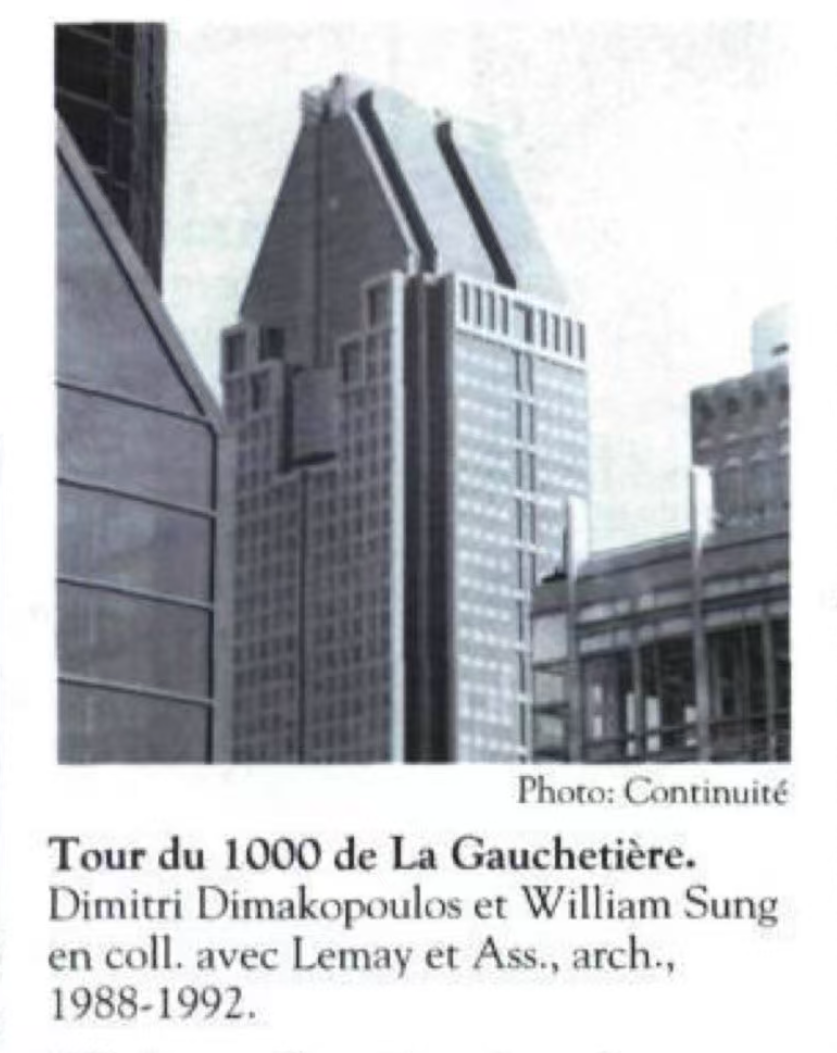
\includegraphics[width=6cm]{!tour_du_1000_deLa_Gauchetiere_250331_thumbnail_picture_(602).png}

\newpage

从小，父母经常给我们灌输的价值观就是：``一定要好好读书，找一个高薪、稳定、不太辛苦的工作，这样年纪大了就能享受轻松的生活了。''因此春节回乡时，亲戚也往往会以收入去评价你。

但随着我工作越久就越来越发现，当收入可以满足家庭的基本需求后，赚钱不再是唯一的追求。其他方面的追求，如工作是否促进自我成长、是否具挑战性和获得满足感等，更为重要。

例如我的二叔William
Sung.，他1933年出生，从小喜欢画画，我还记得看过他的水彩画，很好看。因为他的父母经历过被日军占领3年8个月的日子，都希望子女进政府当公务员，收入稳定有退休金。所以他从香港理工毕业后进政府当卫生检查官。1961年，虽然父母极力反对，他拿着McGill
U的录取信，坐船经日本到加拿大，开始在Montreal读建筑。因为没有父母资助，为节省开支，开始时只能吃罐头、面包，与其他香港同学合租在一间很小的单间。他擅长手工绘制建筑设计图、透视图，在大二开始已经有客户付费请他画图，渐渐有了积蓄，甚至买车，毕业后加入Dimakopoulos
\& Partners，成为合伙人，实现了他的梦想。

所以自己必须有明确清晰的目标，才能不悔此生。企业也类似，所以企业家必须清楚企业的具体标：\\
``5年10年后，希望公司会有什么成就？''

有些企业只有盈利，收入等财务（可量化）目标，但卓越的企业除了这些财务目标以外，更重要有更高的理想和愿景，才能吸引有抱负，有能力的人才加入。（企业的成功还是靠人才。）\\
有些公司为每个岗位设定了KPI，考核结果将直接影响年终奖或晋升。但在与员工的讨论中发现，即使团队成员的KPI全部达标，但整体结果（如成本、质量）却未必理想。所以，如果管理者只追求可量化的指标，而忽视了责任心、团队协作等难以量化的因素，反而会损害整体业务。

例如，某公司每月会选出一位``本月之星''员工，并进行表扬，因缺乏客观的量化指标，竟以员工的打卡时间来衡量。所以KPI或``本月之星''等``激励''措施可能会适得其反。

如果在定期高层会议里，大部分时间都是用于关注各员工的KPI指标是否``高分''，而且没有明确公司愿景，企业就会难以持续健康成长。

所以当 Robert Kaplan与David
Norton在1992年提出平衡计分卡时，商务指标只是4类指标之一，其他还包括：

\begin{itemize}
\tightlist
\item
  从客户视角的指标（客户如何看我们？）
\item
  公司内部业务指标（公司内部卓越之处）
\item
  创新与成长的指标
\end{itemize}


